\documentclass[11pt,a4paper]{article}
%%%%% font, language
\usepackage[utf8]{inputenc}
\usepackage[T1]{fontenc}
\usepackage[UKenglish]{babel}
\usepackage{lmodern}
%%%%% figures
\usepackage{subcaption}
\captionsetup[subfigure]{textfont = normalfont, labelfont = bf, format = hang}
\captionsetup[figure]{textfont = normalfont, labelfont = bf, format = hang}
\captionsetup[table]{textfont = normalfont, labelfont = bf, format = hang}
%%%%% images
\usepackage{graphicx}
\usepackage{pdflscape} % horizontal pages
%%%%% references, quoting
\usepackage[german=quotes]{csquotes}
\usepackage{hyperref}
%%%%% layout
\usepackage[left=2.5cm,right=3cm,top=3cm,bottom=3cm]{geometry}
%%%%%%%%%%
%%%%% own commands
\newcommand{\function}[1]{\texttt{#1}}
\newcommand{\argument}[1]{\texttt{#1}}
\newcommand{\class}[1]{\texttt{#1}}
\newcommand{\enum}[1]{\texttt{#1}}
\newcommand{\package}[1]{\texttt{#1}}
\newcommand{\toolname}{\textit{linteddata}}
%%%%%%%%%%
\begin{document}
\begin{center}
\begin{LARGE}
\textbf{How to add a new validator to \toolname}
\end{LARGE}
\end{center}
\hrule
\tableofcontents
\bigskip
\hrule
%
\section{Structure}
%
\begin{itemize}
	\item describe the structure of this document
\end{itemize}
%
\section{General architecture}
%
In this section at first the architecture is displayed. 
Additionally some of the classes and their functionality are explained.  
\\ 
The general structure of the classes, used to implement the \toolname , is displayed in figure~\ref{fig:general_architecture:class_diagram}. 
The classes belong to three different packages: 
\begin{description}
	\item[checks:] This package contains all the validators. 
	\item[JUnitXML:] All classes in this package are used to build the structure of \cite{JUnitXML_ibm}. 
	\item[Main:] The classes from this package are used to execute the tool. 
\end{description}
%
The different classes in the package \package{checks} are described in section~\ref{sec:check_types}. 
In general all of these classes have a \function{execute} that must be implemented. 
Each of the abstract classes overwrites the \function{execute} of its superclass, except for \class{FileCheck} as the first check. 
\class{Check} is a superclass of \class{FileCheck} and used to capture the attributes of a check. 
It can be used to extend the tool later with different types of checks. 
\\
Each of the \class{FileChecks} has one level it applies to, this could also be modelled via the subclass relation, but with the enum \enum{Level}, the user can pass as an argument what kind of validations he wants to execute. 
A new validator mustn't have the \enum{Level} \enum{ALL}, this value is only for the user input. 
Also each one has a \enum{TargetLanguage}. 
This attribute is used to assign the validator to the corresponding Testsuite in the result. 

The abstract subclasses of the different levels each implement the abstract \texttt{execute} method of its superclass. 
In these implementations the argument, that is not \argument{failureDescription}, is further processed and along with the \argument{failureDescription} passed to the new abstract method \function{execute}.
\\
The package \package{JUnitXML} contains classes that are needed to represent the elements from \cite{JUnitXML_ibm}. 
To prevent misunderstandings, elements of \textit{Testsuites} are represented with instances of the class \class{TestsuiteManager}. 
When adding a new validator, no changes need to be done to this package. 

The \enum{Severity} has the three values \enum{ERROR, WARN} and \enum{INFO}. 
Where \enum{ERROR} is used for critical failures that must be fixed to ensure correctness and functionality. 
\enum{WARN} represents failures that are non critical but should be fixed for correct behaviour. 
The weakest value is \enum{INFO} which is for non critical failures that don't affect the correctness but should be fixed.   
\\
The \function{main}-method is contained in \class{LintedData}. 
Within this class the command-line arguments are processed and a new instance of \class{Runner} is created. 
\class{Runner} executes the selected checks and stores the result to the destination file. 
When a new validator is added, it must be added to the method \function{Runner.createAllChecks}, there are no further changes needed. 
%
\begin{landscape}
\begin{figure}[tb]
	\centering
	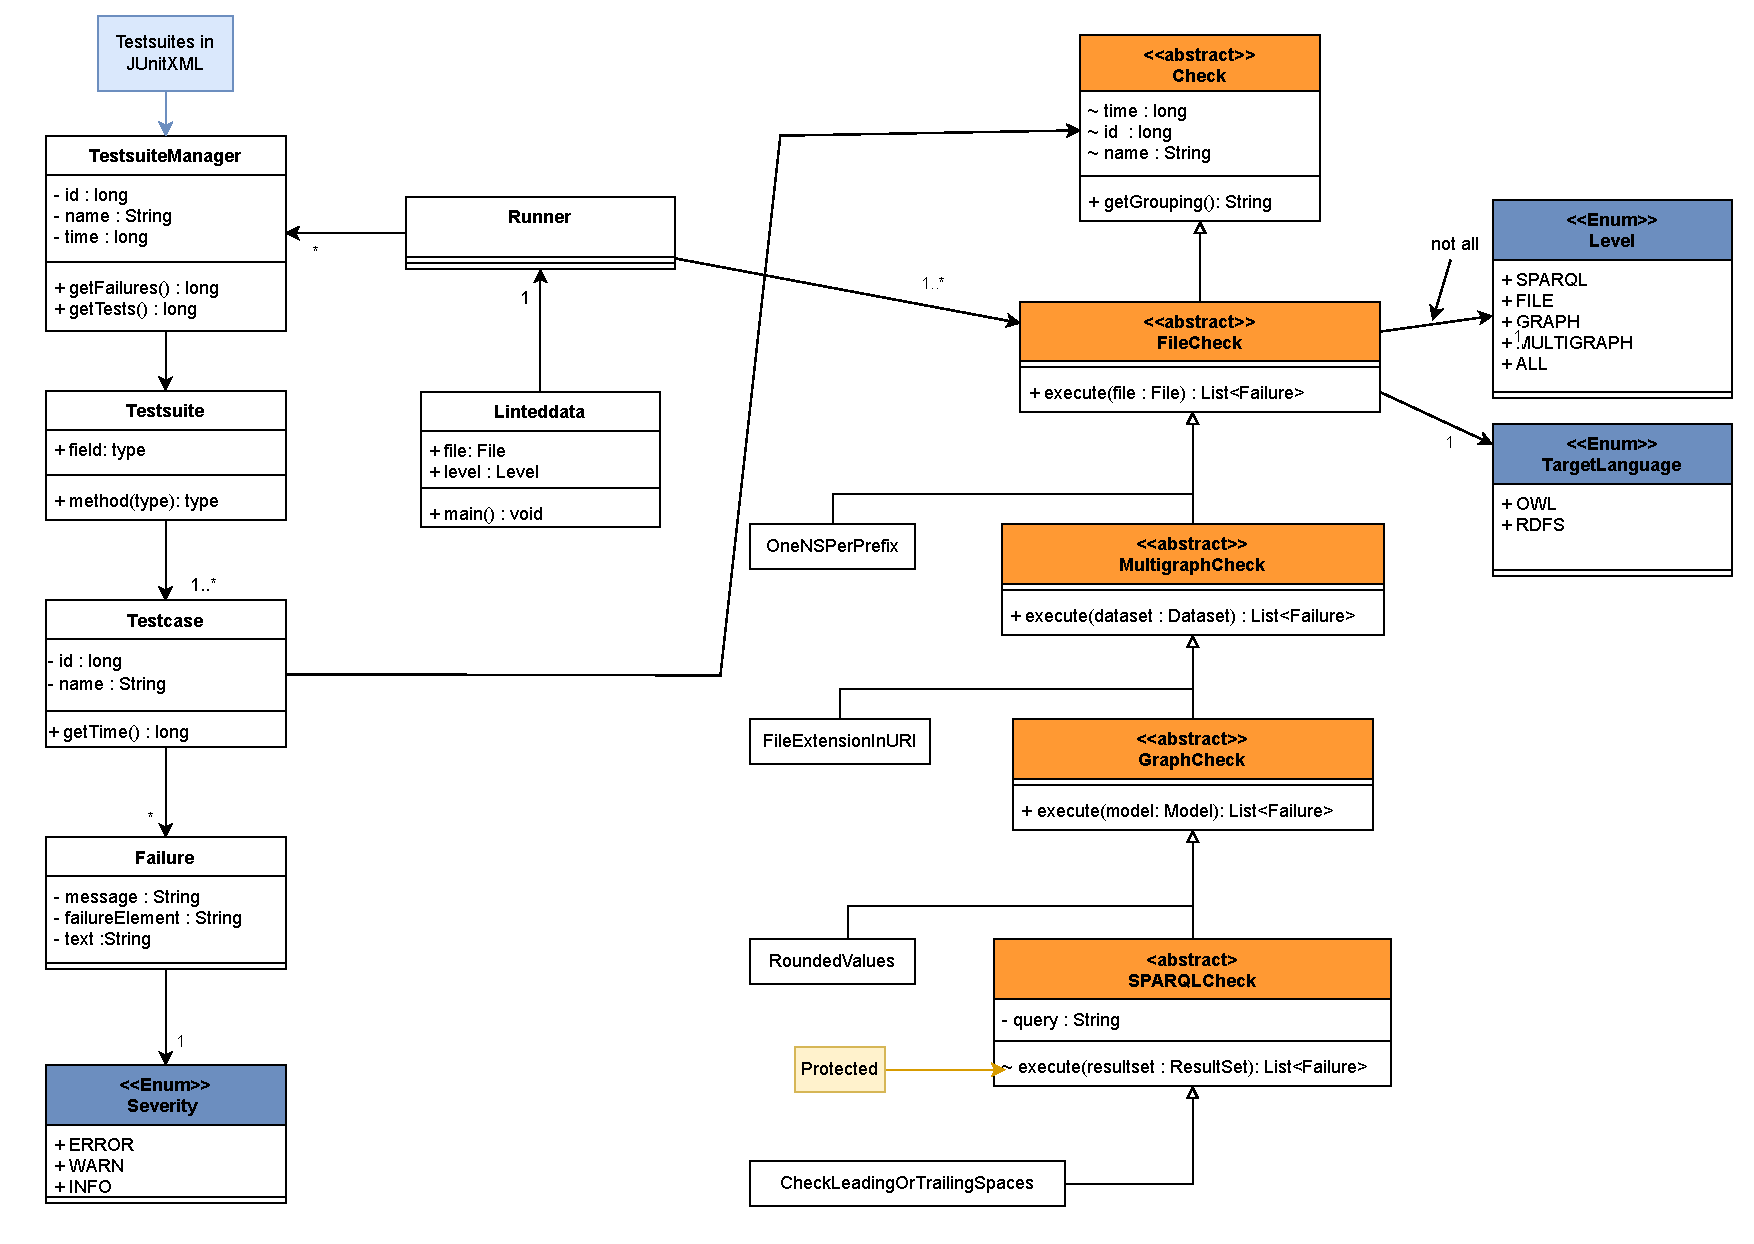
\includegraphics[width=\textwidth]{../graphics/class_diagram.pdf}
	\caption{Class diagram of \toolname .}
	\label{fig:general_architecture:class_diagram}
\end{figure}
\end{landscape}
%
In the following section the classes of the package \package{check} are described more in detail. 
\begin{itemize}
	\item image of the class diagram
	\item should the classes be described more in detail?
\end{itemize}
%
\section{Check types}
\label{sec:check_types}
%
In this section the different types of validators are explained. 
The aim of this section is it, to understand, when to implement which type of check. 

As seen in the class diagram (figure~\ref{fig:general_architecture:class_diagram}), the different types of validators are implemented as subclass from \class{Check}. 

\class{FileCheck} is the first \enquote{real} check that applies to the structure of the tool. 
All non abstract subclasses of this class need to process the file in its raw format. 
The failures detected in those classes can't be detected after parsing the file into a Jena dataset \cite{apache_jena}. 
\\
A validator should be realised as a subclass of \class{MultiGraphCheck} if the problem can be detected after parsing the file, but it is necessary to have access to all models contained in the dataset. 
\\
When a problem affects only a single model from Jena contained in the dataset. 
At this level, it is not possible to access any other model. 
If this is necessary, the validator should be a subclass of \class{MultiGraphCheck}. 
\\
Although implementing a validator as a subclass of \class{SPARQLCheck} might not be the best efficient solution, it should be the superclass to choose. 
If the validator is implemented as SPARQL query, this query can be reused in other frameworks as well. 
 
\begin{itemize}
	\item describe the different types of test
	\item SPARQL checks might be implemented more efficient as a different type, but should be implemented as them $\rightarrow$ can be used in other frameworks 
	\item multi graph level 
	\begin{itemize}
		\item file parsed as dataset
		\item information extracted from all models 
	\end{itemize}
	\item graph level 
	\begin{itemize}
		\item executed on default model and all named models
		\item check always performs on only one model at the same time $\rightarrow$ no information about other models at this point
	\end{itemize}
	\item SPARQL level
	\begin{itemize}
		\item executed on a single model 
		\item query = string $\rightarrow$ attribute
		\item \function{execute} $\rightarrow$ only processing of the query result into failures
	\end{itemize}		 
\end{itemize}
%
\section{Implementation of a new validator}
\begin{enumerate}
	\item choose a corresponding level 
	\item implementation of the constructor
	\begin{itemize}
		\item description of the attributes
		\item choose severity
	\end{itemize}
	\item implementation of the \function{execute} 
	\begin{itemize}
		\item how to customise \argument{failureDescription}
		\item 
	\end{itemize}
	\item test check
	\begin{itemize}
		\item JUnit Test
		\item test the \enquote{lowest} \function{execute} function
	\end{itemize}
	\item add test to the list of all checks
	\begin{itemize}
		\item add check in \function{Runner.createAllChecks()}
	\end{itemize}
\end{enumerate}
%
\section{Example}
\begin{itemize}
	\item documentation of creating a check
\end{itemize}
\end{document}
